
\begin{figure}[t]
        \begin{subfigure}[b]{0.32\textwidth}
        \centering
        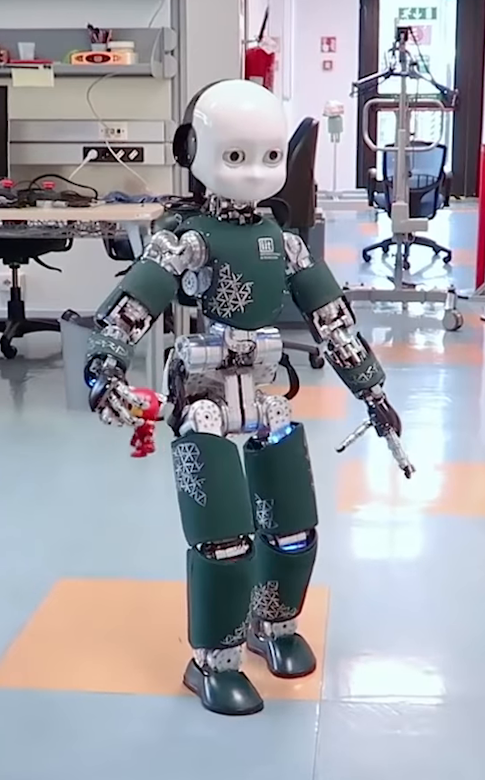
\includegraphics[width=\columnwidth]{chapter_simplified_benchmarking/figures/step1.png}
    \end{subfigure}
    \hfill
           \begin{subfigure}[b]{0.32\textwidth}
        \centering
        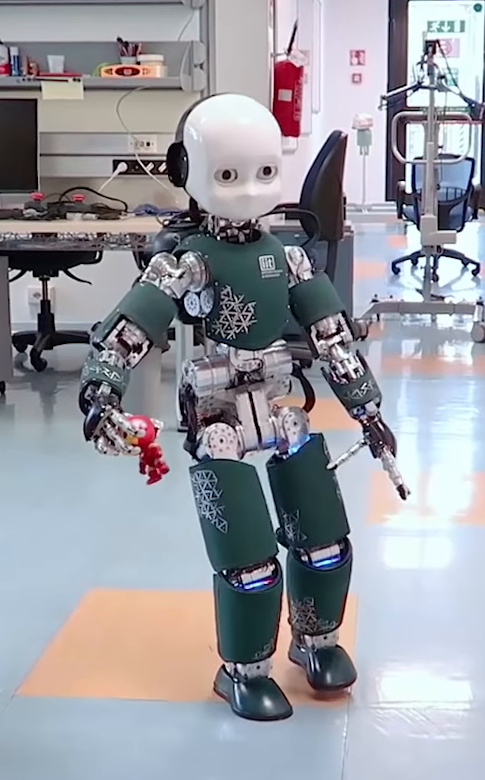
\includegraphics[width=\columnwidth]{chapter_simplified_benchmarking/figures/step2.png}
    \end{subfigure}
    \hfill
           \begin{subfigure}[b]{0.32\textwidth}
        \centering
        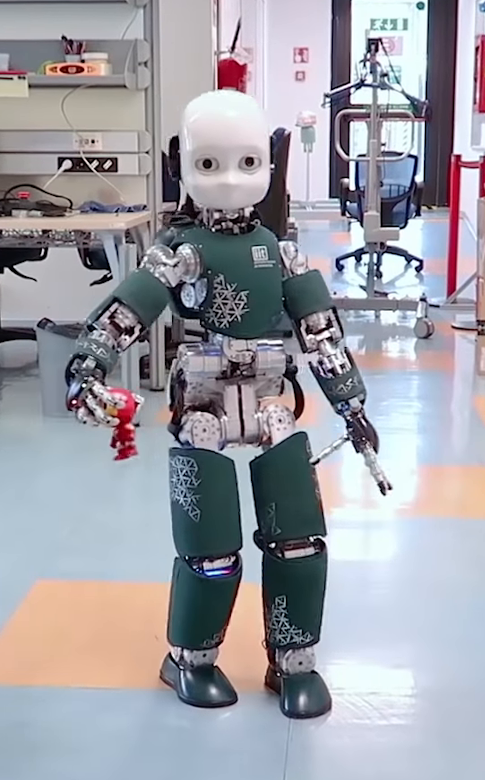
\includegraphics[width=\columnwidth]{chapter_simplified_benchmarking/figures/step3.png}
    \end{subfigure}
    \caption{The iCub robot walks with the 3 layer controller architecture of Figure~\ref{fig:three-layer-simplified-benchmarking}.}
    \label{fig:icub_walking_simplified}
\end{figure}

\section{Results}
\label{sec:results_simplified_benchmarking}
In this section, we present experiments obtained with several implementations of the simplified model controllers, namely: the \emph{instantaneous} and the \emph{predictive} controllers.

To benchmark the different simplified model controllers, we test the algorithms on the iCub humanoid robot v2.7 -- Section~\ref{sec:icub2.7}. We attach the simplified control layer to the three-layer controller architecture shown in Figure~\ref{fig:three-layer}. In this framework, the whole-body control layer implements the kinematics-based whole-body QP presented in section~\ref{sec:ik_qp}. Figure~\ref{fig:icub_walking_simplified} shows the humanoid robot iCub walking with the simplified models controller presented in this chapter.

The control architecture runs on the iCub head's computer, namely a 4-th generation Intel \textsuperscript{\tiny\textregistered} Core i7 @ $\SI{1.7}{\giga \hertz}$. In any of its implementations, the architecture takes (on average) less than $\SI{3}{\milli \second}$ to evaluate its output. The code is open source completely developed in C++: \href{https://github.com/robotology/walking-controllers}{\texttt{https://github.com/robotology/walking-controllers}}. The MPC problem presented in Section~\ref{predictive-control} is solved using the OSQP~\citep{Stellato2018} library~\footnote{Since our code is  written in pure C++, the QP problem is written by means of \texttt{osqp-eigen} a C++ wrapper for OSQP \href{https://github.com/robotology/osqp-eigen}{\texttt{https://github.com/robotology/osqp-eigen}}}.


Table~\ref{tab:max_velocity} summarizes the maximum velocities achieved using the different implementations of the control architecture. In particular, the labels \emph{instantaneous} and \emph{predictive} mean that the associated layer generates its output considering inputs and references either at the single time $t$ or for a time window, respectively. The labels, \emph{velocity} and \emph{position} control, instead, mean that the layer outputs are either desired joint velocities or position, respectively -- see Section~\ref{subsubsec-pos-vel-control}. 

\begin{table}[b]
    \centering
    \caption{Maximum forward straight walking velocities achieved using different implementations of the control architecture.
    }
    \begin{tabular}{cc|c}
         \begin{tabular}{@{}c@{}}Simplified Model  Control\end{tabular} &
         \begin{tabular}{@{}c@{}}Whole-Body QP Control\end{tabular} &
         \begin{tabular}{@{}c@{}}Max Straight Velocity (m/s)\end{tabular}\\
        \hline
        Predictive  & Velocity  &  0.1563\\
        Predictive  & Position  & 0.1645\\
        Instantaneous  & Velocity  &  0.1809\\
        Instantaneous  & Position  & 0.3372
    \end{tabular}
    \label{tab:max_velocity}
\end{table}

Let us remark that all the implemented control architectures exploit the controller presented in Section~\ref{ZMP-CoM-Controller} to attempt the stabilization of the desired center of pressure and desired center of mass position and velocity. The performance of this controller is highly dependent on the gains $K_{zmp}$ and $K_{com}$. In particular, we observed that the gains in achieving good tracking during standing and walking were not the same. For this reason, we implemented a gain-scheduling technique depending on whether the robot is walking or standing. The transition between the two sets of gains is smoothed with a minimum jerk trajectory \citep{Pattacini2010}.


To compare the simplified models controllers, we decided to perform two main experiments. These two experiments represent the maximum robot velocity that has been achieved with all architectures and the maximum velocity achieved with a specific architecture only -- see Table~\ref{tab:max_velocity}. That is, 
\begin{itemize}
    \item[-] \textbf{Experiment 1}: a forward robot speed of $\SI{0.1563}{\meter \per \second}$;
    \item[-] \textbf{Experiment 2}: a forward robot speed of $\SI{0.3372}{\meter \per \second}$.
\end{itemize}

\begin{figure}[t]
    \centering
    \begin{myframe}{Instantaneous + Position Control}
        \centering
    \begin{subfigure}[b]{0.49\textwidth}
        \centering
        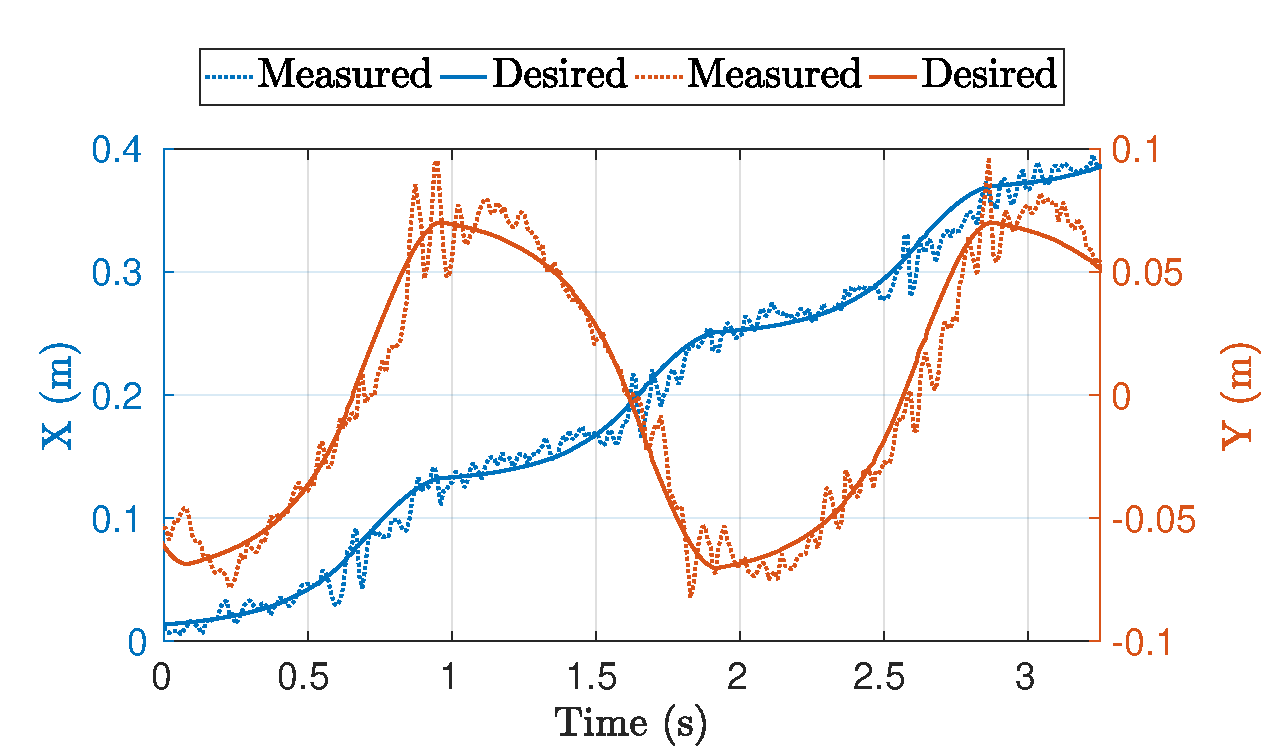
\includegraphics[width=\textwidth]{chapter_simplified_benchmarking/figures/inst_pos-min_vel-dcm.pdf}
        \caption{DCM}
        \label{fig:inst_pos-min_vel-dcm}
    \end{subfigure}
    \hfill
    \begin{subfigure}[b]{0.49\textwidth}
        \centering
        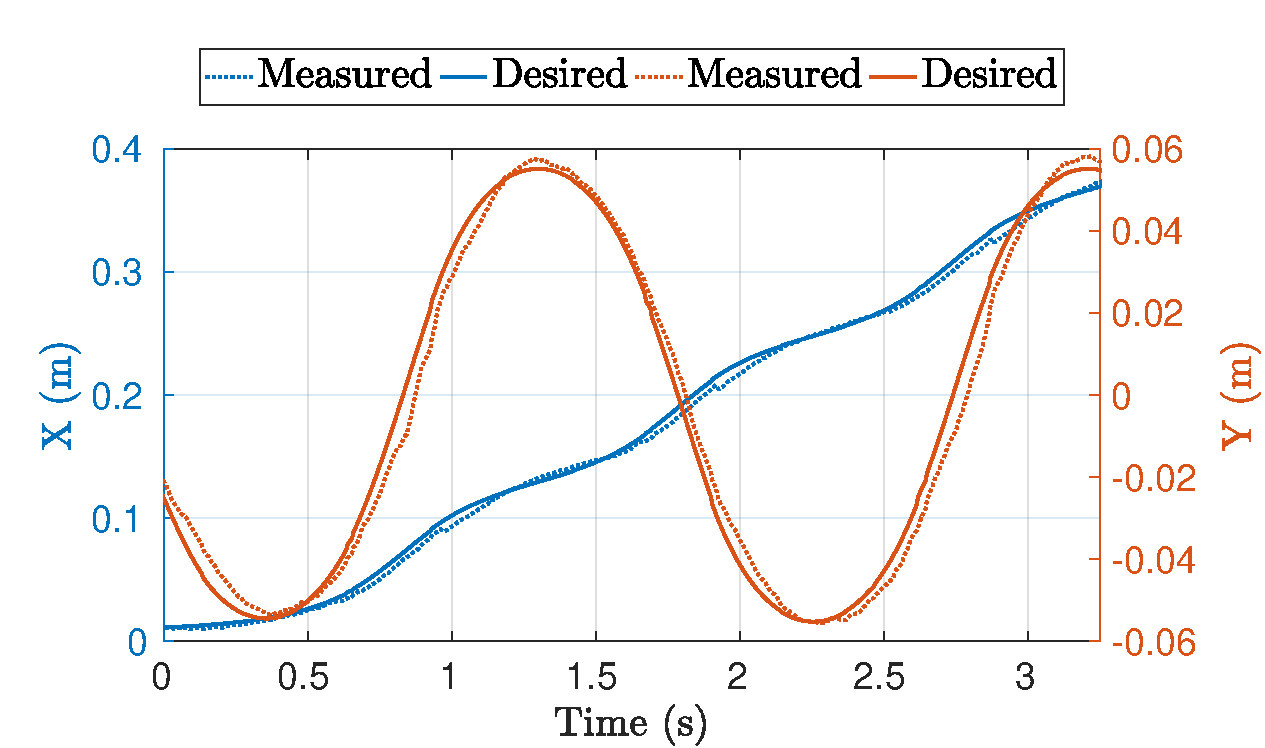
\includegraphics[width=\textwidth]{chapter_simplified_benchmarking/figures/inst_pos-min_vel-com.pdf}
        \caption{CoM}
        \label{fig:inst_pos-min_vel-com}
    \end{subfigure}
    \hfill
    \begin{subfigure}[b]{0.49\textwidth}
        \centering
        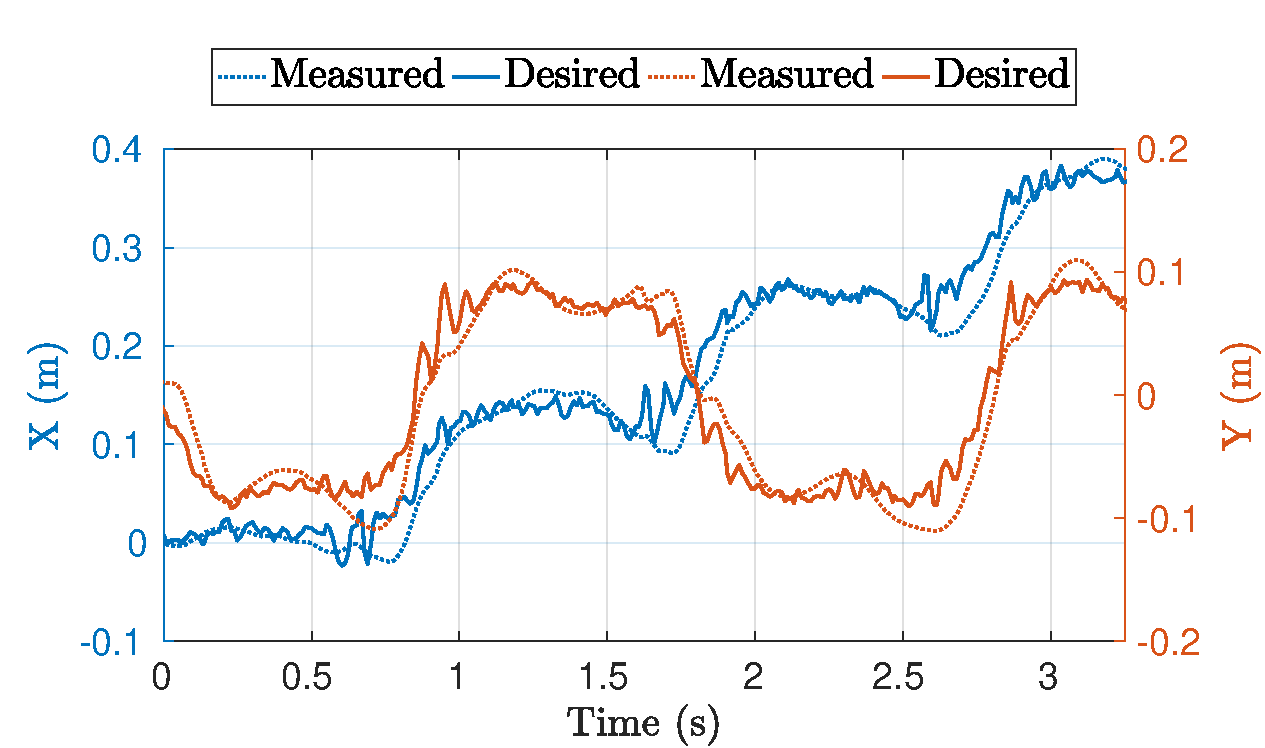
\includegraphics[width=\textwidth]{chapter_simplified_benchmarking/figures/inst_pos-min_vel-zmp.pdf}
        \caption{ZMP}
        \label{fig:inst_pos-min_vel-zmp}
    \end{subfigure}
    \end{myframe}
    \caption{Tracking of the DCM (a), CoM (b) and ZMP (c) using the instantaneous controller with the whole-body controller as position control. Walking velocity:  $\SI{0.19}{\meter \per \second}$.}
\end{figure}

\begin{figure}[t]
    \begin{myframe}{Predictive + Position Control}
     \centering
    \begin{subfigure}[b]{0.49\textwidth}
        \centering
        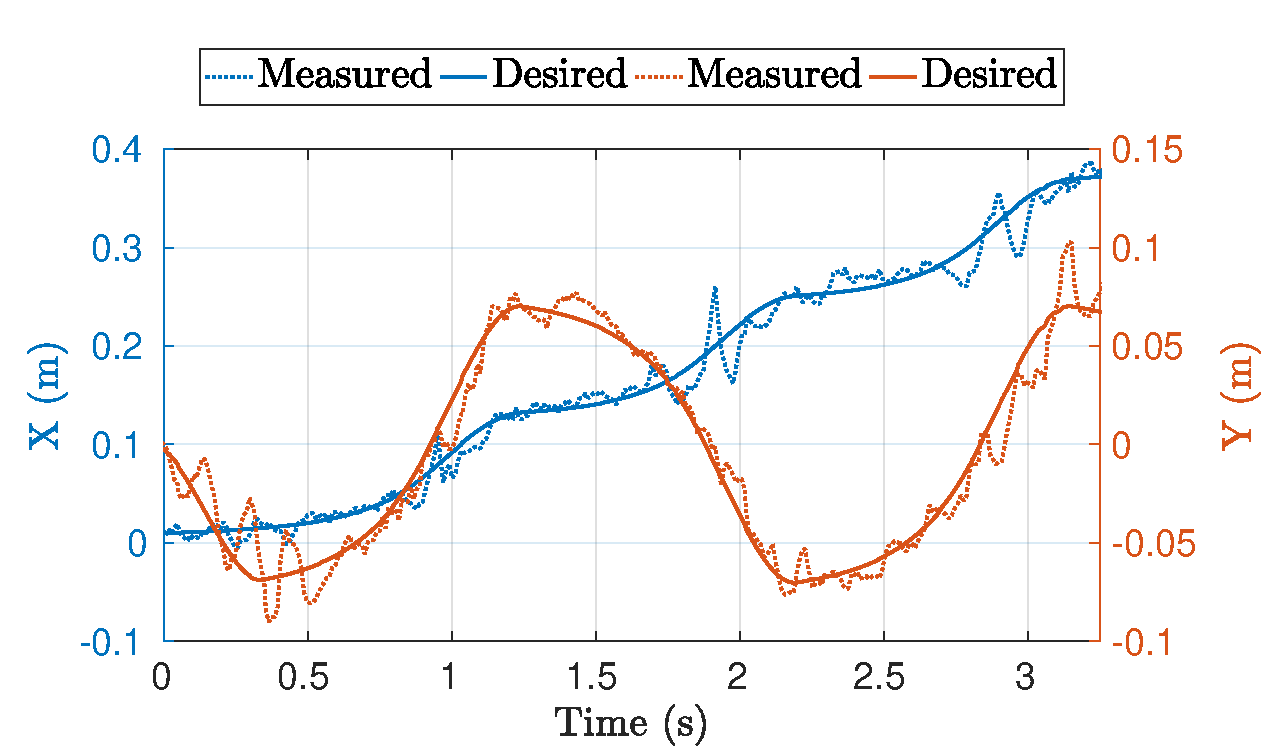
\includegraphics[width=\textwidth]{chapter_simplified_benchmarking/figures/mpc_pos-min_vel-dcm.pdf}
        \caption{DCM}
        \label{fig:mpc_pos-min_vel-dcm}
    \end{subfigure}
    \hfill
    \begin{subfigure}[b]{0.49\textwidth}
        \centering
        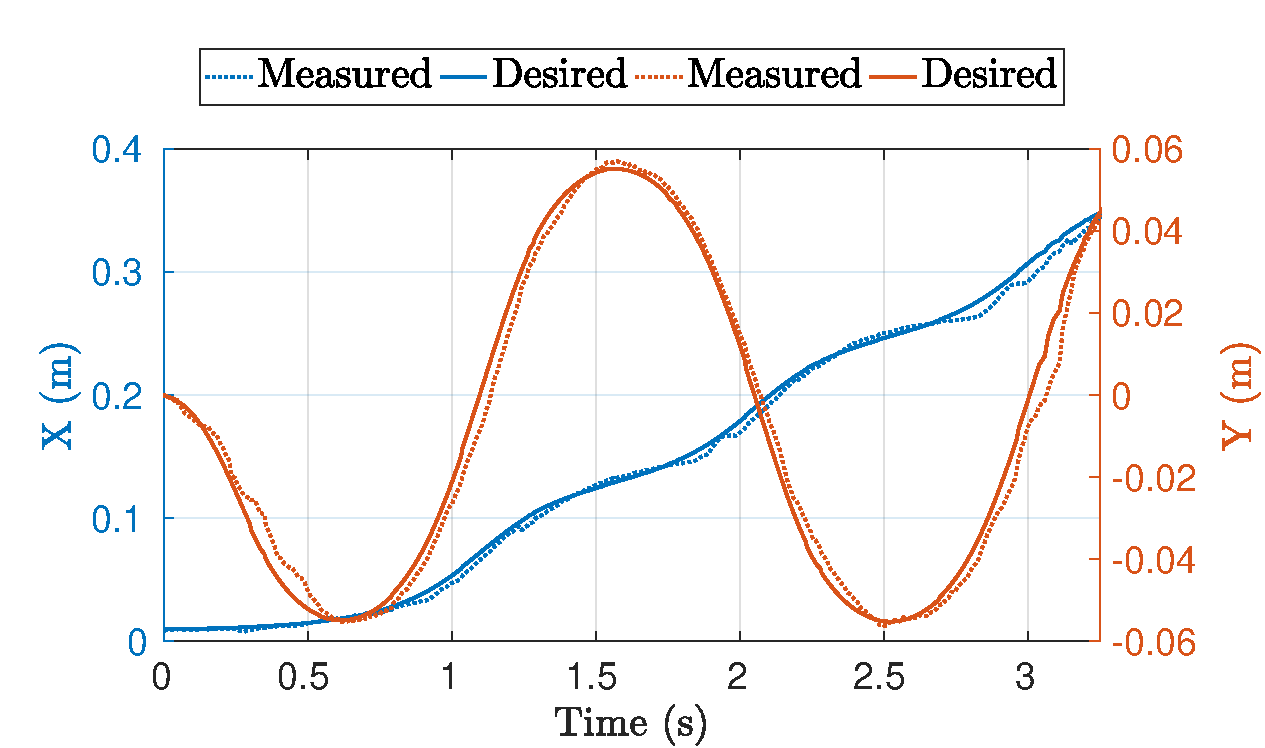
\includegraphics[width=\textwidth]{chapter_simplified_benchmarking/figures/mpc_pos-min_vel-com.pdf}
        \caption{CoM}
        \label{fig:mpc_pos-min_vel-com}
    \end{subfigure}
         \begin{subfigure}[b]{0.49\textwidth}
        \centering
        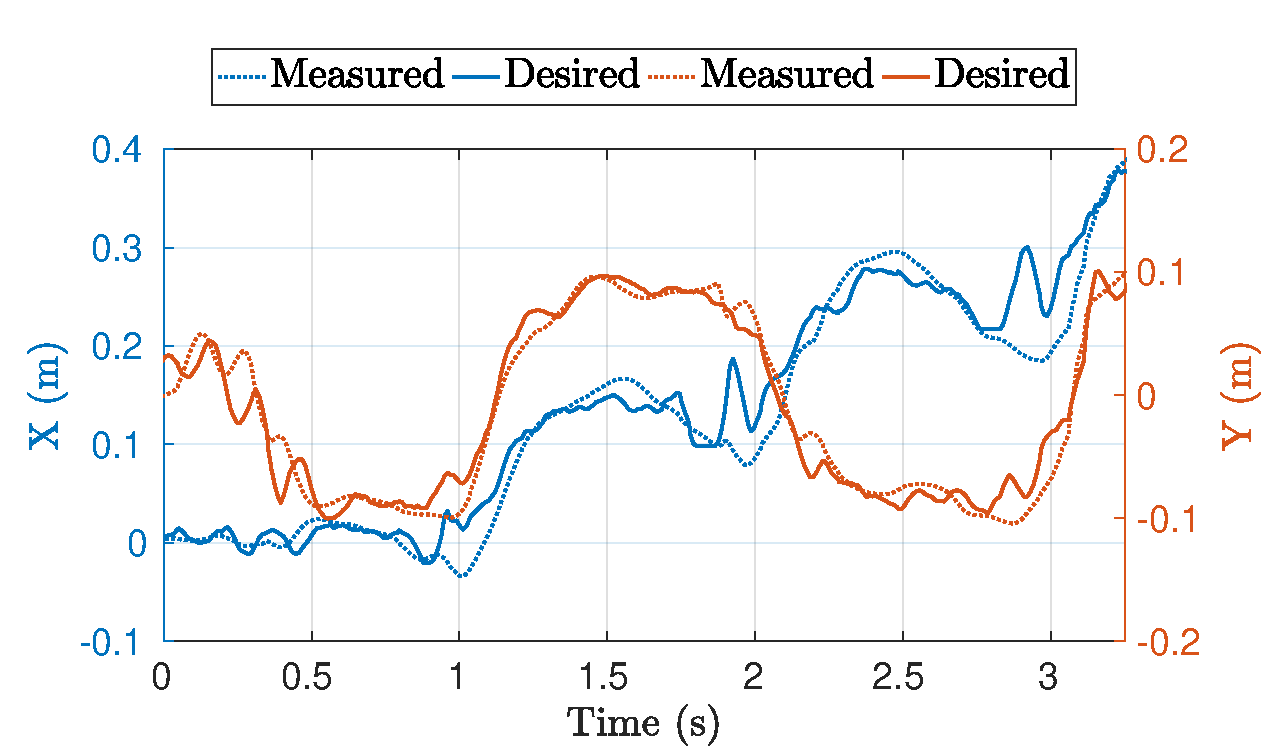
\includegraphics[width=\textwidth]{chapter_simplified_benchmarking/figures/mpc_pos-min_vel-zmp.pdf}
        \caption{ZMP}
        \label{fig:mpc_pos-min_vel-zmp}
    \end{subfigure}
    \end{myframe}
    \caption{Tracking of the  DCM (a), CoM (b) and ZMP (c) using the MPC and the whole-body controller as position control. Walking velocity:  $\SI{0.19}{\meter \per \second}$.}
\end{figure}
\begin{figure}[t]
     \vspace*{-0.1cm}
    \begin{myframe}{Instantaneous + Position Control}
    \centering
        \begin{subfigure}[b]{0.49\textwidth}
        \centering
        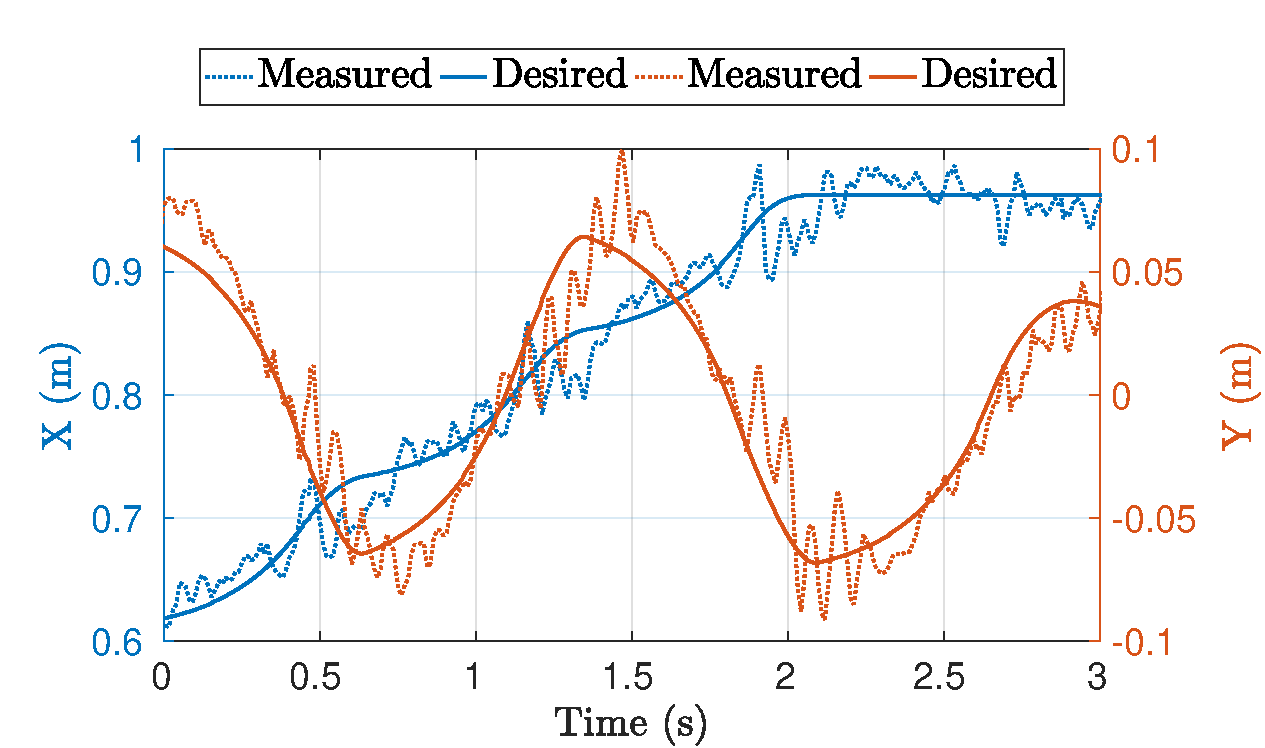
\includegraphics[width=\textwidth]{chapter_simplified_benchmarking/figures/inst_pos-max_vel-dcm.pdf}
        \caption{DCM}
        \label{fig:inst_pos-max_vel-dcm}
    \end{subfigure}
    \hfill
     \begin{subfigure}[b]{0.49\textwidth}
        \centering
        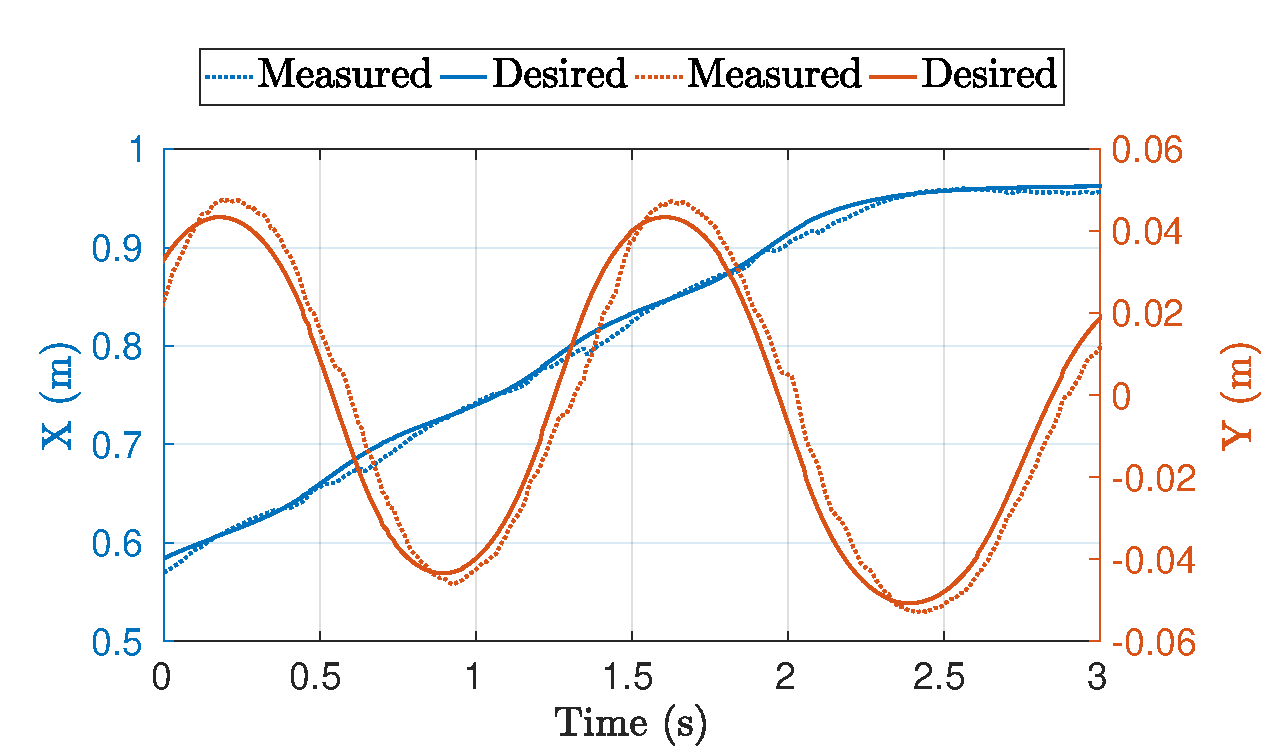
\includegraphics[width=\textwidth]{chapter_simplified_benchmarking/figures/inst_pos-max_vel-com.pdf}
        \caption{CoM}
        \label{fig:inst_pos-max_vel-com}
    \end{subfigure}
    \hfill
    \begin{subfigure}[b]{0.49\textwidth}
        \centering
        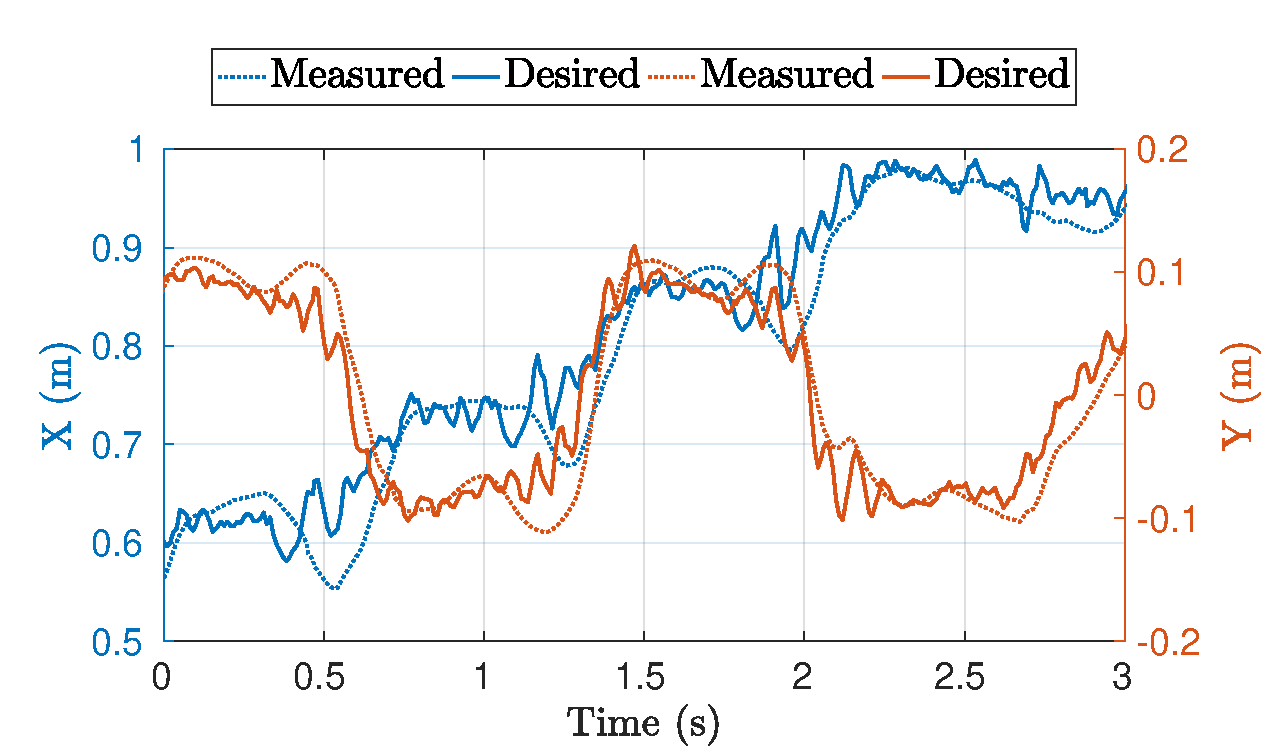
\includegraphics[width=\textwidth]{chapter_simplified_benchmarking/figures/inst_pos-max_vel-zmp.pdf}
        \caption{ZMP}
        \label{fig:inst_pos-max_vel-zmp}
    \end{subfigure}
    \end{myframe}
    \caption{Tracking of the DCM (a), CoM (b) and ZMP (c) with the instantaneous and whole-body QP control as position.  Walking velocity: $\SI{0.41}{\meter \per \second}$.}
\end{figure}
\begin{figure}[t]
    \begin{myframe}{Predictive + Position Control}
    \centering
    \begin{subfigure}[b]{0.49\textwidth}
        \centering
        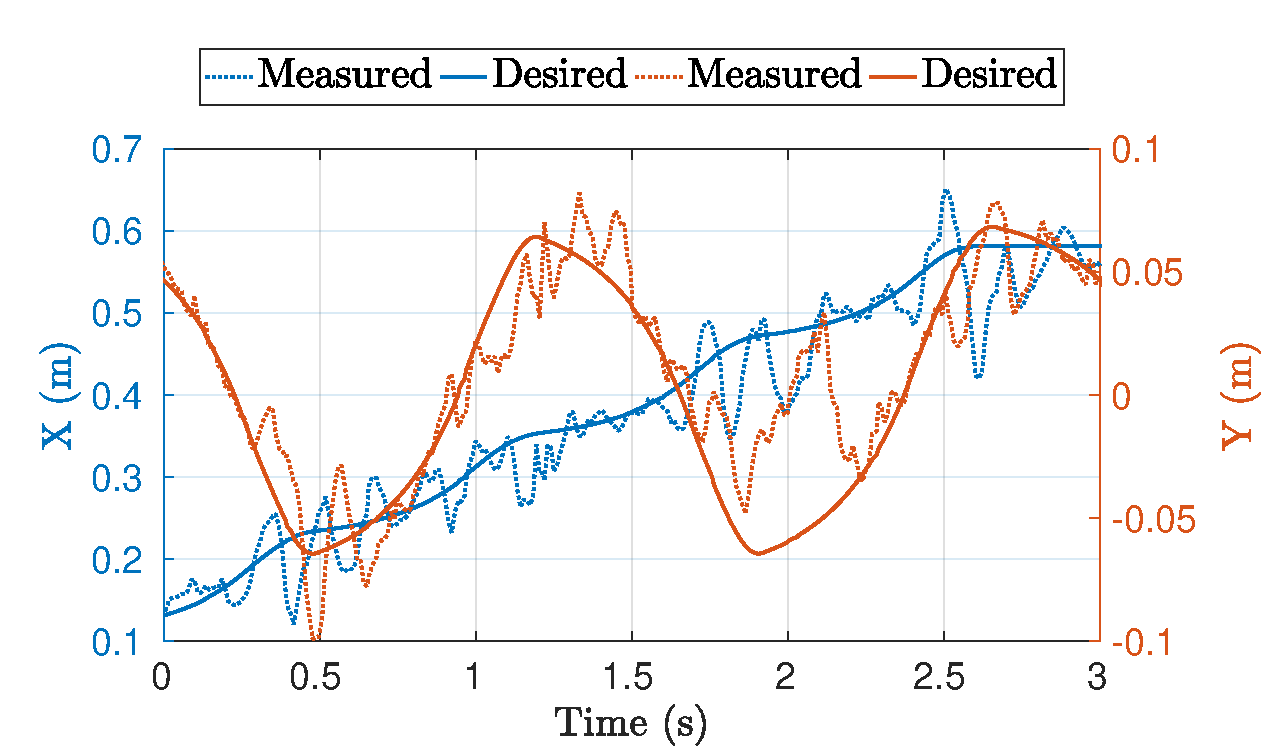
\includegraphics[width=\textwidth]{chapter_simplified_benchmarking/figures/mpc_pos-max_vel-dcm.pdf}
        \caption{DCM}
        \label{fig:mpc_pos-max_vel-dcm}
    \end{subfigure}
    \hfill
     \begin{subfigure}[b]{0.49\textwidth}
        \centering
        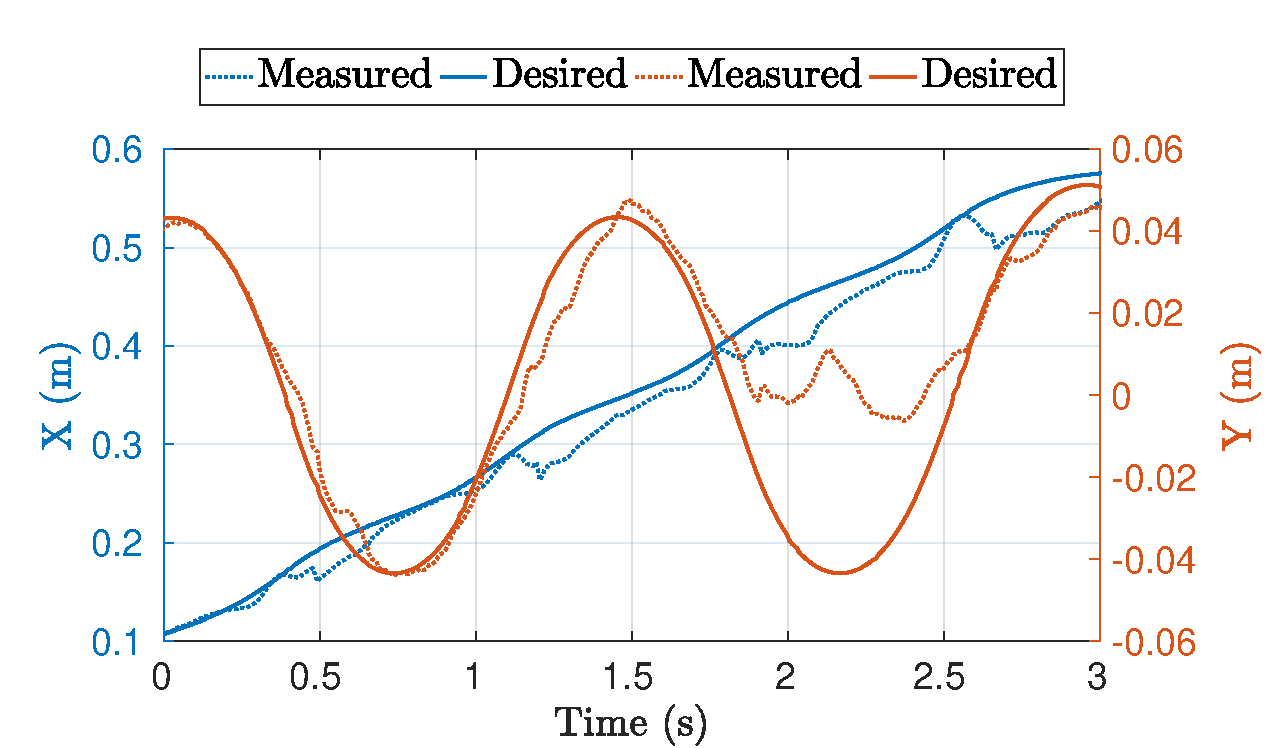
\includegraphics[width=\textwidth]{chapter_simplified_benchmarking/figures/mpc_pos-max_vel-com.pdf}
        \caption{CoM}
        \label{fig:mpc_pos-max_vel-com}
    \end{subfigure}
    \hfill
    \begin{subfigure}[b]{0.49\textwidth}
        \centering
        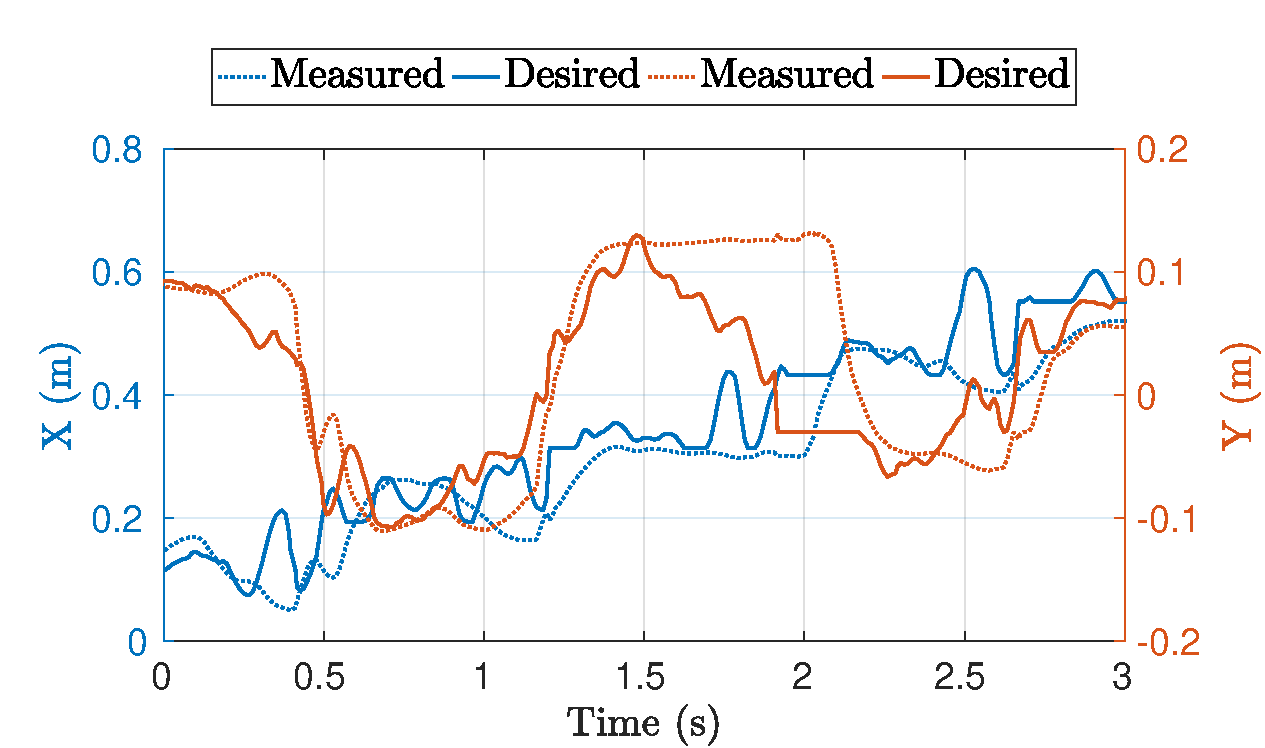
\includegraphics[width=\textwidth]{chapter_simplified_benchmarking/figures/mpc_pos-max_vel-zmp.pdf}
        \caption{ZMP}
        \label{fig:mpc_pos-max_vel-zmp}
    \end{subfigure}
    \end{myframe}
    \caption{Tracking of the  DCM (a), CoM (b) and ZMP (c) with the predictive and whole-body QP control as position control. At $t\approx \SI{2}{\second}$, the robot falls down.  Walking velocity: $\SI{0.41}{\meter \per \second}$.}
    \vskip-0.5cm
\end{figure}

We compare the control laws~\eqref{eq:reactive_dcm} and~\eqref{eq:mpc_solution_simplified}, which both generate a (desired) center of pressure that attempts to stabilize the desired DCM. To simplify the comparison, the controller of the \emph{whole-body QP layer} is kept fixed in this section, and we show and discuss only the results when the robot is position controlled. A complete comparison of the kinematics-based whole-body controllers is presented in Section~\ref{sec:wbc_experimental_results}.
In the following experiments, we set the time horizon of the predictive control to $\SI{2}{\second}$.

\subsection{Experiment 1: a forward robot speed of 0.1563 m s$^{\text{-1}}$}
Figures \ref{fig:inst_pos-min_vel-dcm} and \ref{fig:mpc_pos-min_vel-dcm} show the DCM tracking performances obtained with the instantaneous and predictive controllers, respectively. Both controllers seem to show good tracking performances, and the DCM error is kept below $\SI{5}{\centi \meter}$ in both cases. Note, however, that the instantaneous controller induces faster variations of the measured DCM. This contributes to the overall higher vibrations of the robot. One of the reasons for this variation is that the instantaneous controller~\eqref{eq:reactive_dcm} injects a (desired) center of pressure proportional to the measured DCM, which in turn contains the center of mass velocity. To mitigate this, we may filter the joint velocities appropriately. However, in our case, the joint velocities were not filtered to avoid delays in the measured DCM. Our experience showed that adding a filter to joint velocities is not an easy task, and we did not find the right trade-off for obtaining overall performance improvements. 

Figures~\ref{fig:inst_pos-min_vel-com} and \ref{fig:mpc_pos-min_vel-com} present CoM tracking performances, which are mainly dependent on the ZMP-CoM controller~\eqref{eq:ZMP_controller}. This controller receives the desired DCM values from the \emph{simplified model control} layer, which are obtained with the instantaneous or predictive controllers. In both cases, the CoM error is kept below $\SI{2}{\centi \meter}$. Figures~\ref{fig:inst_pos-min_vel-zmp} and~\ref{fig:mpc_pos-min_vel-zmp} represent the ZMP tracking performance, which is still mainly dependent on the ZMP-CoM controller~\eqref{eq:ZMP_controller}. It is important to note that the desired ZMP is smoother when the \emph{simplified model control} uses the predictive law~\eqref{eq:mpc_solution_simplified} to generate it. Indeed, this is a tunable property that depends on the associated weight in the cost function of the MPC problem. Although this smoother behavior contributes to less robot vibrations, overall robot performance became less reactive and, consequently, less robust to robot falls. Although the extensive hand-made tuning, we were not able to increase the robot velocity when the \emph{simplified model control} used the predictive law~\eqref{eq:mpc_solution_simplified}. 

\subsection{Experiment 2: a forward robot speed of 0.3372 m s$^{\text{-1}}$}
At a robot's desired walking speed of $\SI{0.3372}{\meter \per \second}$, there is initially no significant difference between the DCM tracking obtained with instantaneous and predictive control laws -- see Figures~\ref{fig:mpc_pos-max_vel-dcm} and~\ref{fig:inst_pos-max_vel-dcm} for $t < \SI{1.5}{\second}$. However, fast robot walking velocities require fast variations of the desired CoM and ZMP. This fast variation degrades the performance of the predictive controller around $t = \SI{1.5}{\second}$ -- see Figure~\ref{fig:mpc_pos-max_vel-zmp}. Clearly, these bad performances, in turn, induce poor tracking of the DCM shown in Figure~\ref{fig:mpc_pos-max_vel-dcm} at $t\approx \SI{2}{\second}$, and consequently the robot falls. At this point, one is tempted to increase the gain $K_\text{ZMP}$ of the controller~\eqref{eq:ZMP_controller}, which shall induce a better tracking of the ZMP. Unfortunately, this leads to higher robot oscillations induced by the noise on the estimated ZMP. And, as a consequence, the robot falls. 

We can conclude that the \emph{predictive simplified control} is much less robust than the \emph{instantaneous simplified control} with respect to ZMP tracking errors. Adding a low-pass filter to the ZMP measurement may improve the overall performance. However, in our case, adding filters led to slower system response and, consequently, to the robot falling.


